\documentclass[conference]{IEEEtran}

\usepackage{multirow}
\usepackage{booktabs}
\usepackage[T1]{fontenc}
\usepackage[utf8]{inputenc}
\usepackage{cite}
\usepackage{amsmath,amssymb,amsfonts}
\usepackage{graphicx}
\usepackage{booktabs}
\usepackage{hyperref}

\begin{document}

\title{Fault Detection and Isolation - Report}

\author{\IEEEauthorblockN{Emmeran Colot}}

\maketitle

\section{Introduction}

This report covers the different implementations of fault detection and isolation methods for discrete-time systems. It shows and analyses the results obtained based on the theoretical explanations given by Prof. M. Kinnaert in the \textit{Model-Based and Data-Driven Fault Detection and Isolation} course.

The discrete-time state space model is given by
\begin{equation}
    \begin{cases}
        x[k+1] = A x[k] + B u[k] + E_d d[k] + E_f f[k] \\
        y[k] = C x[k] + D u[k] + G_d d[k] + G_f f[k]
    \end{cases}
    \label{eq:ss_model}
\end{equation}
where $x \in \mathbb{R}^{n \times 1}$ is the state, $u \in \mathbb{R}^{m \times 1}$ the input to the system, $y \in \mathbb{R}^{p \times 1}$ the output of the system, $d \in \mathbb{R}^{n_d \times 1}$ the disturbance and $f \in \mathbb{R}^{n_f \times 1}$ the fault. The exact values for those matrices are given in Appendix \ref{appendix:exact_model}.

\section{Parity relations based method}

\subsection{Overview of the method}

Based on the state space representation (\ref{eq:ss_model}), $y[k]$ can be expressed as a function of the state at time instance $k-s$ and the input, disturbance and fault from time instance $k-s$ up to $k$. This was derived by recurrence and the resulting equation, in a matrix form, is
\begin{equation}
    Y_s(k) = \Theta_s x(k-s) + T_s^u U_s(k) + T_s^d D_s(k) + T_s^f F_s(k).
    \label{eq:parity_relation}
\end{equation}
The "\textit{signal matrices}" are built as follows
\begin{equation}
    Y_s(k) = \begin{bmatrix}
        y[k-s] \\ \vdots \\ y[k]
    \end{bmatrix}
    \qquad \cdots \qquad
    F_s(k) = \begin{bmatrix}
        f[k-s] \\ \vdots \\ f[k]
    \end{bmatrix},
\end{equation}
and the "\textit{weight matrices}":
\begin{equation}
    \begin{gathered}
        \Theta_s = \begin{bmatrix}
            C \\ C A \\ \vdots \\ C A^s
        \end{bmatrix}
        \quad , \quad
        T_s^u = \begin{bmatrix}
            D & \mathbf{0} & \cdots & \mathbf{0} \\
            C B & D & \ddots & \vdots \\
            \vdots & \ddots & \ddots & \mathbf{0} \\
            C A^{s-1} B & \cdots & C B & D
        \end{bmatrix} \\
        T_s^{d/f} = \begin{bmatrix}
            G_{d/f} & \mathbf{0} & \cdots & \mathbf{0} \\
            C E_{d/f} & G_{d/f} & \ddots & \vdots \\
            \vdots & \ddots & \ddots & \mathbf{0} \\
            C A^{s-1} E_{d/f} & \cdots & C E_{d/f} & G_{d/f}
        \end{bmatrix}
    \end{gathered}
\end{equation}
Because of their nature, disturbances are unknown (stochastic noise, nonlinearities, unmeasured input signal, ...) and the state is often not measured. To only keep from (\ref{eq:parity_relation}) the fault and the measured signals, they are split from the other terms and both sides of the equation is then multiplied by $\Omega_s$. 

The unknown side of the equation can then be cancelled with a clever choice for $\Omega_s$, i.e. a basis of the left null space of $\left[\Theta_s \quad T_s^d\right]$:
\begin{equation}
    \Omega_s \left(Y_s(k) - T_s^u U_s(k) - T_s^f F_s(k)\right) = \mathbf{0}.
\end{equation}

It is worth mentioning the existence condition for $\Omega_s$, which depends on the rank of the matrix to cancel:
\begin{equation}
    \text{rank}\begin{bmatrix}
        \Theta_s & T_s^d
    \end{bmatrix} < (s+1) p
    \label{eq:existence_Omega_s}
\end{equation}

This leads to the definition of the residual vector, which is equal to $\mathbf{0}$ in case there is no fault and is computed by
\begin{equation}
    r[k] = \Omega_s \left(Y_s(k) - T_s^u U_s(k)\right).
    \label{eq:residual_vector}
\end{equation}

\subsection{Fault detection}

Applied to a system with 1 input and 2 outputs, a simulation has been done with $s = 2$. It contains a sinusoidal disturbance and a fault on the sensors. Fig. \ref{fig:system_evolution} shows what is computed by the simulation in a case where no fault is present.

\begin{figure}[htbp]
    \centering
    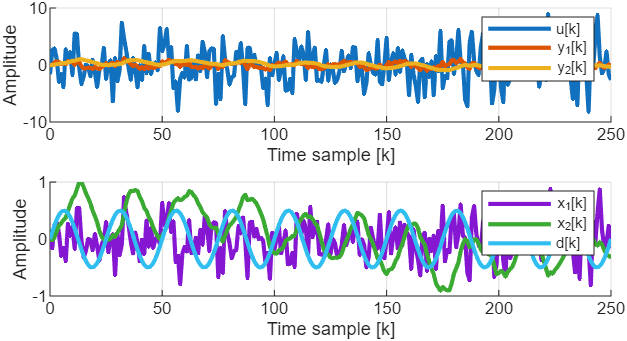
\includegraphics[width=0.48\textwidth]{../Matlab/ParityMethods/System Evolution.png}
    \caption{Measured signals (top) and internal signals (bottom) in a faultless scenario.}
    \label{fig:system_evolution}
\end{figure}

The simulation is ran with a constant bias error on each of the two sensors and the resulting residual vector norm is shown on Fig. \ref{fig:step_fault}.

\begin{figure}[htbp]
    \centering
    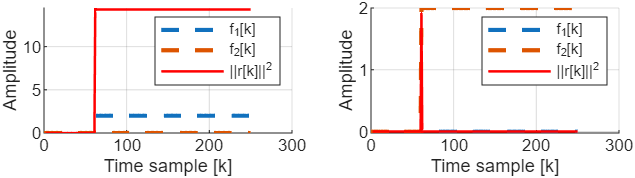
\includegraphics[width=0.48\textwidth]{../Matlab/ParityMethods/Step Fault.png}
    \caption{Applied fault (on state 1 on the left plot and state 2 on the right plot) and resulting residual.}
    \label{fig:step_fault}
\end{figure}

The residual on the right subplot indicates that the fault can be detected but is forgotten after a few samples. This is because the second state integrates the input, meaning a constant error will not be detected. On the other hand, the first state is simply amplifying the input. A constant difference between the expected output and the measured one is therefore easily detected.

For the same reason, a ramp-shaped fault will generate a ramp shaped-residual when applied on the first state and a constant residual in the other case, as shown on Fig. \ref{fig:ramp_fault}.

\begin{figure}[htbp]
    \centering
    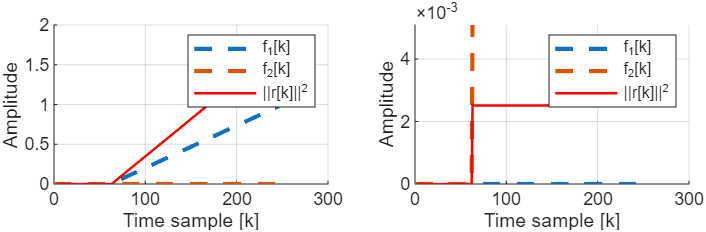
\includegraphics[width=0.48\textwidth]{../Matlab/ParityMethods/Ramp Fault.png}
    \caption{Applied fault (on state 1 on the left plot and state 2 on the right plot) and resulting residual. The second fault looks like a step due to the scale difference between the residual vector norm and the fault signal.}
    \label{fig:ramp_fault}
\end{figure}

\subsection{Fault Isolation}

To isolate the fault, i.e. determine which is the faulty sensor, residuals must be crafted by considering some faults as disturbances using a incidence matrix. Because on the existence condition on the left null space of $\left[\Theta_s \quad T_s^d\right]$ given by (\ref{eq:existence_Omega_s}), a residual generally cannot be built to control a single fault.

To understand how fault isolation works, the system is slightly modified by adding a second sensor on the first output. Three distinct residuals are then built, each targeting all but one fault according to the following incidence matrix:

\begin{table}[htbp]
    \centering
    \begin{tabular}{c|ccc}
        & $f_1$ & $f_2$ & $f_3$ \\
        \hline
        $r_1$ & 0 & $\times$ & $\times$ \\
        $r_2$ & $\times$ & 0 & $\times$ \\
        $r_3$ & $\times$ & $\times$ & 0 \\
    \end{tabular}
\end{table}

To generate $r_1$, the disturbance matrices $E_d$, $G_d$ and the fault matrices $E_f$, $G_f$ are modified. By moving some columns from the fault matrices to the disturbance matrices as follows,
\begin{equation}
    \begin{cases}
        E_d = \begin{bmatrix}
            E_{d_1}
        \end{bmatrix} \\
        E_f = \begin{bmatrix}
            E_{f_1} & E_{f_2} & E_{f_3}
        \end{bmatrix} \\
        G_d = \begin{bmatrix}
            G_{d_1}
        \end{bmatrix} \\
        G_f = \begin{bmatrix}
            G_{f_1} & G_{f_2} & G_{f_3}
        \end{bmatrix}
    \end{cases}
    \quad \Rightarrow \quad \begin{cases}
        E_d = \begin{bmatrix}
            E_{d_1} & E_{f_1}
        \end{bmatrix} \\
        E_f = \begin{bmatrix}
            E_{f_2} & E_{f_3}
        \end{bmatrix} \\
        G_d = \begin{bmatrix}
            G_{d_1} & G_{f_1}
        \end{bmatrix} \\
        G_f = \begin{bmatrix}
            G_{f_2} & G_{f_3}
        \end{bmatrix}
    \end{cases}
\end{equation}

the residual $r_1$ will now only detects faults on the $2^{\text{nd}}$ and $3^{\text{rd}}$ sensors. The same approach allows to generate 3 residuals, and therefore a fault can be isolated by inspecting which residual has not increased.

Fig. \ref{fig:isolation} shows a fault applied on different sensors and the corresponding residuals. Looking at the ones that are activated and combining it with the knowledge of the incidence matrix shows it is working as intended.

\begin{figure}[htbp]
    \centering
    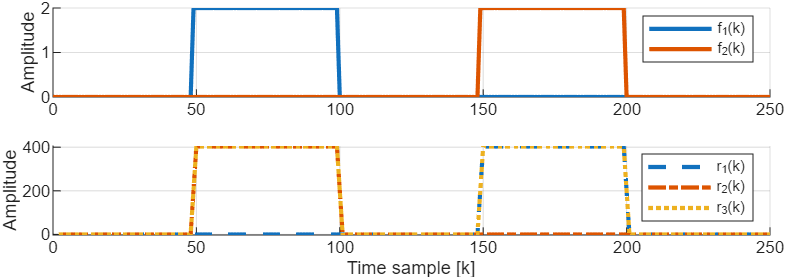
\includegraphics[width=0.48\textwidth]{../Matlab/ParityMethods/Isolation.png}
    \caption{Applied faults (top) and resulting residuals (bottom).}
    \label{fig:isolation}
\end{figure}

If multiple errors occur at the same time, there is no way of determining which sensor is faulty as shown on Fig. \ref{fig:isolation_combined}. As all the residuals are active between the $100^{\text{th}}$ and the $150^{\text{th}}$ samples, faults are still detected but cannot be isolated.

\begin{figure}[htbp]
    \centering
    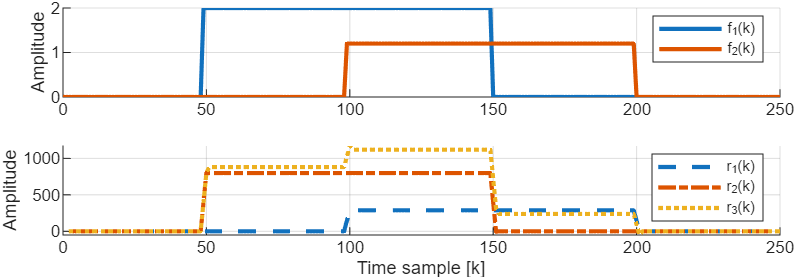
\includegraphics[width=0.48\textwidth]{../Matlab/ParityMethods/Isolation Combined.png}
    \caption{Applied faults (top) and resulting residuals (bottom).}
    \label{fig:isolation_combined}
\end{figure}

\subsection{Redundant sensors}

This section shows how a parity-based approach can be used to detect and isolate faults in a stochastic framework. The studied system is described in Appendix \ref{appendix:pressure_sensors} and two fault detection criterions will be compared: a first one based on the quadratic form of the residual, and the second one derived from the log-likelihood ratio.

\subsubsection{Quadratic criterion}
Starting from the residual computation (\ref{eq:residual_vector}) and taking into account the absence of a state update, $\Omega$ becomes the left null space of $C$ only, and the residual can be expressed as:
\begin{equation}
    \begin{aligned}
        r[k] &= \Omega y[k]\\
        &= \Omega \left(f[k] + \xi[k] \right)
    \end{aligned}
\end{equation}

The variance of the residual can be computed as follows, taking into account $\xi$ is zero-mean.
\begin{equation}
    \mathbb{E}\Big\{ \big(r[k] - \Omega f[k]\big)\big(r[k] - \Omega f[k]\big)^T \Big\} = \Omega R \Omega^T
\end{equation}

This leads to the definition of the normalized residual such that $\tilde{r} \sim \mathcal{N}(0, 1)$.

\begin{equation}
    \label{eq:normalized_residual}
    \begin{gathered}
        \tilde{r}[k] = F y[k]\\
        \text{where} \quad F = \begin{bmatrix}
            F_1 & F_2 & F_3
        \end{bmatrix} = \Big(\Omega R \Omega^T\Big)^{-\frac{1}{2}} \Omega
    \end{gathered}
\end{equation}

A decision layer is then built on top of this residual to estimate when a fault is occurring and when not. For this purpose, a detection measure $d[k]$ is defined based on sum of squares of residuals, meaning $d \sim \chi^2(d_f)$\footnote{$d_f$ is the number of degrees of freedom of variable $d$, here equal to twice the window size.}. Two decision criterions are used here:
\begin{equation}
    \label{eq:decision_criterion}
    d[k] = \begin{cases}
        \tilde{r}_1^2[k] + \tilde{r}_2^2[k], \hspace{2.35cm} \text{the overall criterion}\\
        \sum_{i=0}^{N_w} \tilde{r}_1^2[k-i] + \tilde{r}_2^2[k-i], \quad \text{the windowed criterion}
    \end{cases}
\end{equation}

The threshold value is determined based on this $\chi^2$ distribution and is here chosen to let $1$\% of the samples to be above it. For a measure to be considered faulty, the percentage of residuals above this threshold should be larger than the theoretical $1$\%. 

Fig. \ref{fig:residual_stochastic} shows that a faultless scenario (here with $10^4$ samples) generates around $1$\% of above-threshold residuals, as expected. This number goes up to $\simeq 1.5$\% in this test scenario (fault of $10$\% of the steady state value).

\begin{figure}[htbp]
    \centering
    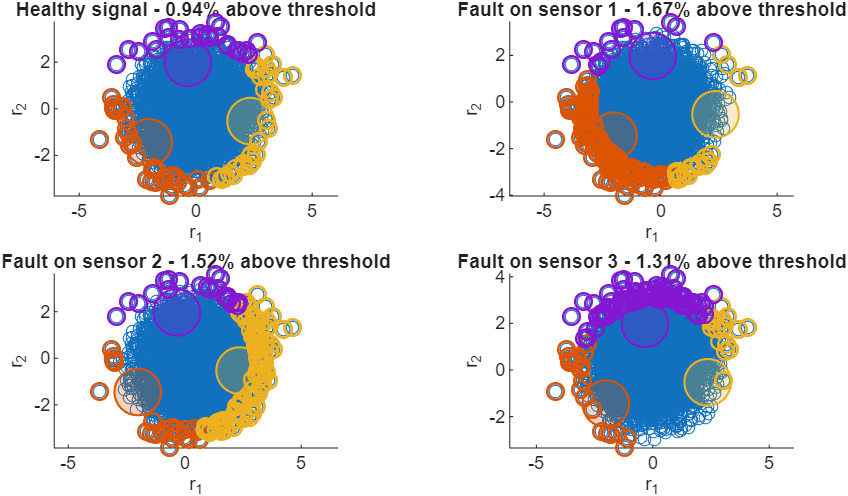
\includegraphics[width=0.48\textwidth]{../Matlab/RedundantSensors/Residual Stochastic.png}
    \caption{Residuals (blue) and fault directions: $F_1$ in orange, $F_2$ in yellow and $F_3$ in purple. Residuals above the threshold are colored with the fault they are attributed to. This used the overall criterion of (\ref{eq:decision_criterion})}
    \label{fig:residual_stochastic}
\end{figure}

Isolation is performed by matching above-threshold residuals to the fault vector $F_i$ they are the closest (angularly). Fig. \ref{fig:residual_stochastic} shows that the faulty sensor is correctly identified.

\subsubsection{GLR}
The Generalized log-Likelihood Ratio (GLR) criterion is based on the Neymann-Pearson test, which is the most powerful test for any chosen type 1 error probability. Using the notation of \ref{appendix:pressure_sensors}, the GLR criterion over a window of $N_w$ samples is defined as follows:
\begin{equation}
    \begin{cases}
        P = \Big( R^{-1} - R^{-1} C \left(C^TR^{-1}C\right)^{-1}C^TR^{-1} \Big)\\
        \ln \hat{\lambda} [k] = y^T[k] P y[k]\\
        \ln \hat{\lambda}_{\text{windowed}} [k] = \sum_{i=0}^{N_w} \ln \hat{\lambda} [k-i]
    \end{cases}
    \label{eq:GLR_algo}
\end{equation}

The threshold is once again determined using the $\xi^2$ distribution with twice the window size as number of degrees of freedom. Tested on a faultless signal, the percentage of samples where the criterion exceeded the threshold were close to the desired type 1 error rate of 1\%.

\subsubsection{Window size impact}

Using the quadratic criterion, it can be seen from (\ref{eq:decision_criterion}) that the overall criterion is equal to the windowed criterion if the window length $N_w$ is set to $1$. Therefore, the decision criterion is compared for a set of window lengths (1, 10, 100 and 500).

\begin{figure}[htbp]
    \centering
    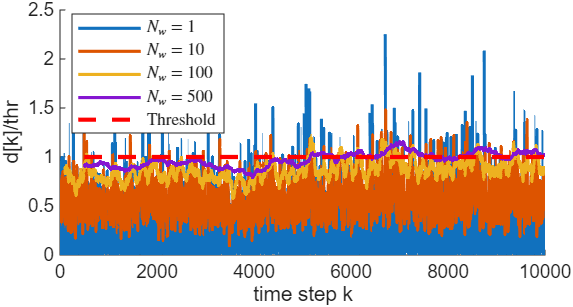
\includegraphics[width=0.48\textwidth]{../Matlab/RedundantSensors/Windowed stochastic residual.png}
    \caption{Decision variable depending on the window length with a fault magnitude 10 times smaller than the steady state. $d[k]$ is scaled by their threshold such that overlapping it with different window size has a meaning.}
    \label{fig:windowed_residual_stochastic}
\end{figure}

Fig. \ref{fig:windowed_residual_stochastic} shows that increasing the window length smoothen $d[k]$, which makes it stick closer to the threshold. Once the default has occurred, almost every sample is detected as being faulty and the above-threshold percentage increases with the window size, as shown in Table \ref{tab:window_above_threshold}.

\begin{table}[htbp]
    \centering
    \caption{Percentage of samples above threshold depending on the window length for the quadratic criterion (\ref{eq:decision_criterion}) and the GLR criterion (\ref{eq:GLR_algo}).}
    \label{tab:window_above_threshold}
    \begin{tabular}{ccc}
        \toprule
        \multirow{2}{*}{Window length $N_w$} & \multicolumn{2}{c}{Above-threshold percentage} \\
        \cmidrule(r){2-3}
                                            & Quadratic & GLR \\
        \midrule
        1   & 1.74\%  & 1.67\%  \\
        10  & 2.75\%  & 2.80\%  \\
        100 & 13.41\% & 13.10\% \\
        500 & 46.51\% & 50.82\% \\
        \bottomrule
    \end{tabular}
\end{table}

The same tests were applied using the GLR criterion, which gave a figure similar to Fig.~\ref{fig:windowed_residual_stochastic} and is therefore not showed. The above-threshold percentage values are also in Table~\ref{tab:window_above_threshold}, showing similar performances to the ones obtained with the quadratic criterion.

\section{Observer based method}

In this section, faults will be detected and isolated using methods based on state estimation. Depending on the type of model, Luenberger estimators or Kalman filters will be applied to build residuals.

The objective is to perform fault detection and isolation on the output signal of a tree-phased signal, which model is derived in Appendix \ref{appendix:three_phased_model}. Because there is no input to the system, all the equations in this section do not contain the input term $u$ nor the related matrices of the state space model $B$ and $D$.

\subsection{Deterministic model}
\label{sec:Luenberger_observer}

Starting from the discrete-time state space model (\ref{eq:ss_model}), it is here considered to be free of any disturbance. A Luenberger observer is then built such that $\hat{x}$ estimates the true state $x$ using
\begin{equation}
    \hat{x}[k+1] = A\hat{x}[k] + L \left(y[k] - C\hat{x}[k]\right).
\end{equation}

The residual is then defined as the difference between the estimated output $\hat{y}$ and the measured one
\begin{equation}
    \begin{aligned}
        &\Leftrightarrow r[k] = y[k] - \hat{y}[k] \\
        &\Leftrightarrow r[k] = y[k] - C \hat{x}[k]
    \end{aligned}
    \label{eq:Luenberger_residual}
\end{equation}

To go towards fault isolation, the $C$matrix is truncated of one or more outputs, which build observers of a subsystem. This allows to detect faults that appear on a specific subset of sensors.

There is a condition on the existence of this observer which is quite obvious: $(A, C_{i, .})$ should be observable, where $C_{i,.}$ represents the $i^{\text{th}}$ row of $C$\footnote{This condition can be weakened as the observer could be built to only observe the observable subsystem.}.

A first set of observers were built using the following incidence matrix:

\begin{table}[htbp]
    \centering
    \begin{tabular}{c|ccc}
        & $f_1$ & $f_2$ & $f_3$ \\
        \hline
        $r_1$ & $\times$ & 0 & 0 \\
        $r_2$ & 0 & $\times$ & 0 \\
        $r_3$ & 0 & 0 & $\times$ \\
    \end{tabular}
\end{table}

Applied on the faulty signal, the measured signals and the residuals are shown on Fig. \ref{fig:fault_present} and the bias on the second signal is clearly identified. The initial estimated state is randomly chosen, which explains why the residuals are not null in the first few samples.

\begin{figure}[htbp]
    \centering
    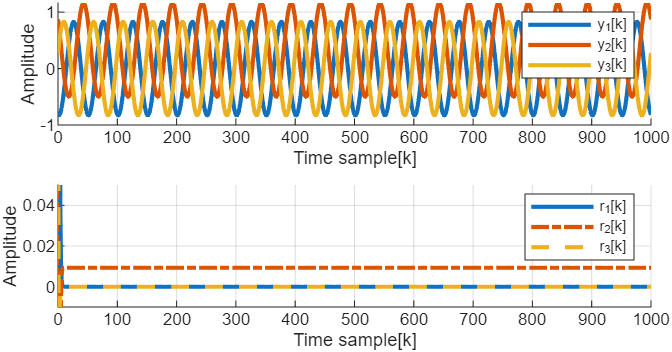
\includegraphics[width=0.48\textwidth]{../Matlab/ObserverMethods/Fault present.png}
    \caption{Measured signals (top) and resulting residuals (bottom).}
    \label{fig:fault_present}
\end{figure}

A different incidence matrix:

\begin{table}[htbp]
    \centering
    \begin{tabular}{c|ccc}
        & $f_1$ & $f_2$ & $f_3$ \\
        \hline
        $r_1$ & 0 & $\times$ & $\times$ \\
        $r_2$ & $\times$ & 0 & $\times$ \\
        $r_3$ & $\times$ & $\times$ & 0 \\
    \end{tabular}
\end{table}

was applied on the same signal and the residuals also allow to isolate the fault, as the $1^{\text{st}}$ and the $3^{\text{rd}}$ residuals are non-zero on Fig. \ref{fig:fault_present_alt}.

\begin{figure}[htbp]
    \centering
    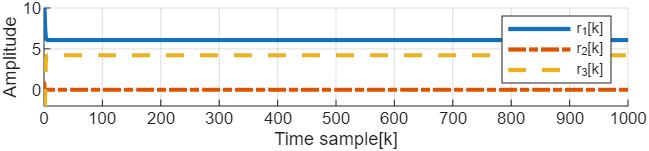
\includegraphics[width=0.48\textwidth]{../Matlab/ObserverMethods/Fault present alt.png}
    \caption{Residuals with the alternative incidence matrix.}
    \label{fig:fault_present_alt}
\end{figure}

\subsection{Stochastic model}

For cases where uncorrelated white gaussian noise is present, it is known that the Kalman filter is the optimal state estimator. The fault isolation method is therefore modified.

The estimated state $\hat{x}$ is obtained by
\begin{equation}
    \hat{x}[k+1] = A \hat{x}[k] + K[k] \left(y[k] - C \hat{x}[k]\right),
\end{equation}
which is the basic Kalman state update. The gain $K$ equation and the state variance $\Sigma$ are also kept as usual:
\begin{gather}
    K[k] = A \Sigma[k] C^T \left(C \Sigma[k] C^T + R\right)^{-1} \\
    \Sigma[k+1] = A \Sigma[k] A^T - K[k] C \Sigma[k] A^T
\end{gather}

$R$ is the measurement noise matrix, measured by computing the variance of the difference between the noisy (non-faulty) signal and the perfect one. Note the process noise matrix $Q$ has been removed from the equation as no process noise is present. Finally, the residual is defined just like (\ref{eq:Luenberger_residual}):
\begin{equation}
    r[k] = y[k] - C \hat{x}[k]
\end{equation}

As in Sec. \ref{sec:Luenberger_observer}, different observers can be built by selecting specific rows of the output matrix $C$, effectively selecting outputs on which checking for fault. With a diagonal incidence matrix, the fault isolation algorithm has been tested on a noisy faultless signal on Fig. \ref{fig:fault_present_Kalman} where it can be seen that the mean residuals lay close to zero.

\begin{figure}[htbp]
    \centering
    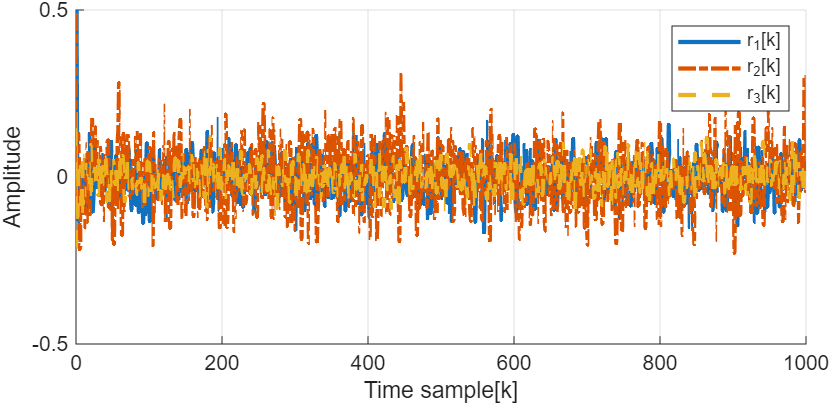
\includegraphics[width=0.48\textwidth]{../Matlab/ObserverMethods/Fault present Kalman.png}
    \caption{Residuals in a faultless scenario.}
    \label{fig:fault_present_Kalman}
\end{figure}

Fig. \ref{fig:fault_present_alt_Kalman} showcases the effectiveness of fault isolation as only the second residual has a non-zero mean.

\begin{figure}[htbp]
    \centering
    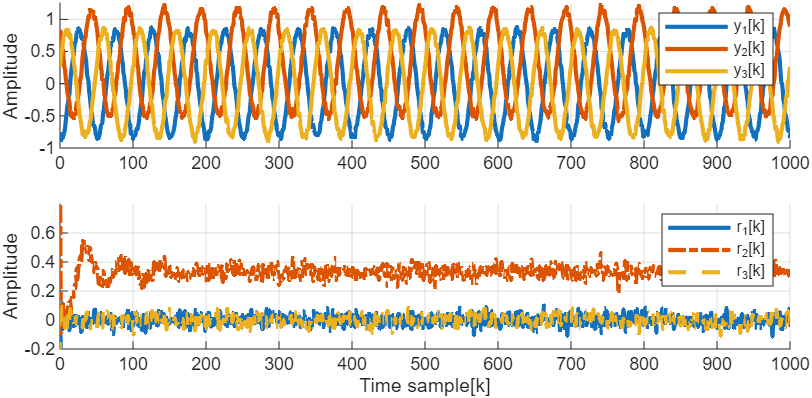
\includegraphics[width=0.48\textwidth]{../Matlab/ObserverMethods/Fault present alt Kalman.png}
    \caption{Measured signal (top) and residuals (bottom).}
    \label{fig:fault_present_alt_Kalman}
\end{figure}

\section{On-line Fault Detection}

On-line fault detection aims at determining the occurrence of a fault and the time at which it occurred on a continuously measured signal. Two algorithms are used here, namely the CUSUM and the GLR, and are described in this section.

The signal on which those algorithms are applied is detailed in Appendix \ref{annex:onlineSystem}.

\subsection{CUSUM}

This algorithm used the cumulative sum, hence its name, of the log-likelihood ratio of a fault occurring on a single data sample:

\begin{equation}
    \begin{cases}
        s[k] = \ln \frac{p_{\text{fault}} (r[k])}{p_{\text{no fault}} (r[k])}\\
        S[k] = \sum_{i=1}^{k} s[k]
    \end{cases}
    \label{eq:CUSUM}
\end{equation}

The maximal value of this cumulative sum $S[k]$ is used as decision function

\begin{equation}
    g[k] = \operatorname{max}_{1 \leq j \leq k} S[j],
\end{equation}

triggered if it exceeds a chosen threshold $h$. The estimated time of default occurrence is found by looking for the first index $m = k-d[k]$ such that $g[m + i] > 0, \forall i \in \{0, \dots, k-m\}$.

Those were the basic formulas but the implementation uses a recursive version to compute the decision $g[k]$ and the detection delay $d[k]$:
\begin{gather}
        g[k] = \sup\Big(0, g[k-1] + s[k]\Big)\\
        d[k] = \begin{cases}
            d[k-1] + 1 \qquad \text{if } g[k-1] > 0\\
            1 \hspace{2.33cm} \text{otherwise}
        \end{cases}
\end{gather}

In our situation, the log-likelihood ratio $s$ can in such case be expressed as

\begin{equation}
    s[k] = \frac{m_1 - m_0}{\sigma^2}\Big(r[k] - \frac{m_1 + m_0}{2}\Big)
    \label{eq:CUSUM_s}
\end{equation}

\begin{figure}[htbp]
    \centering
    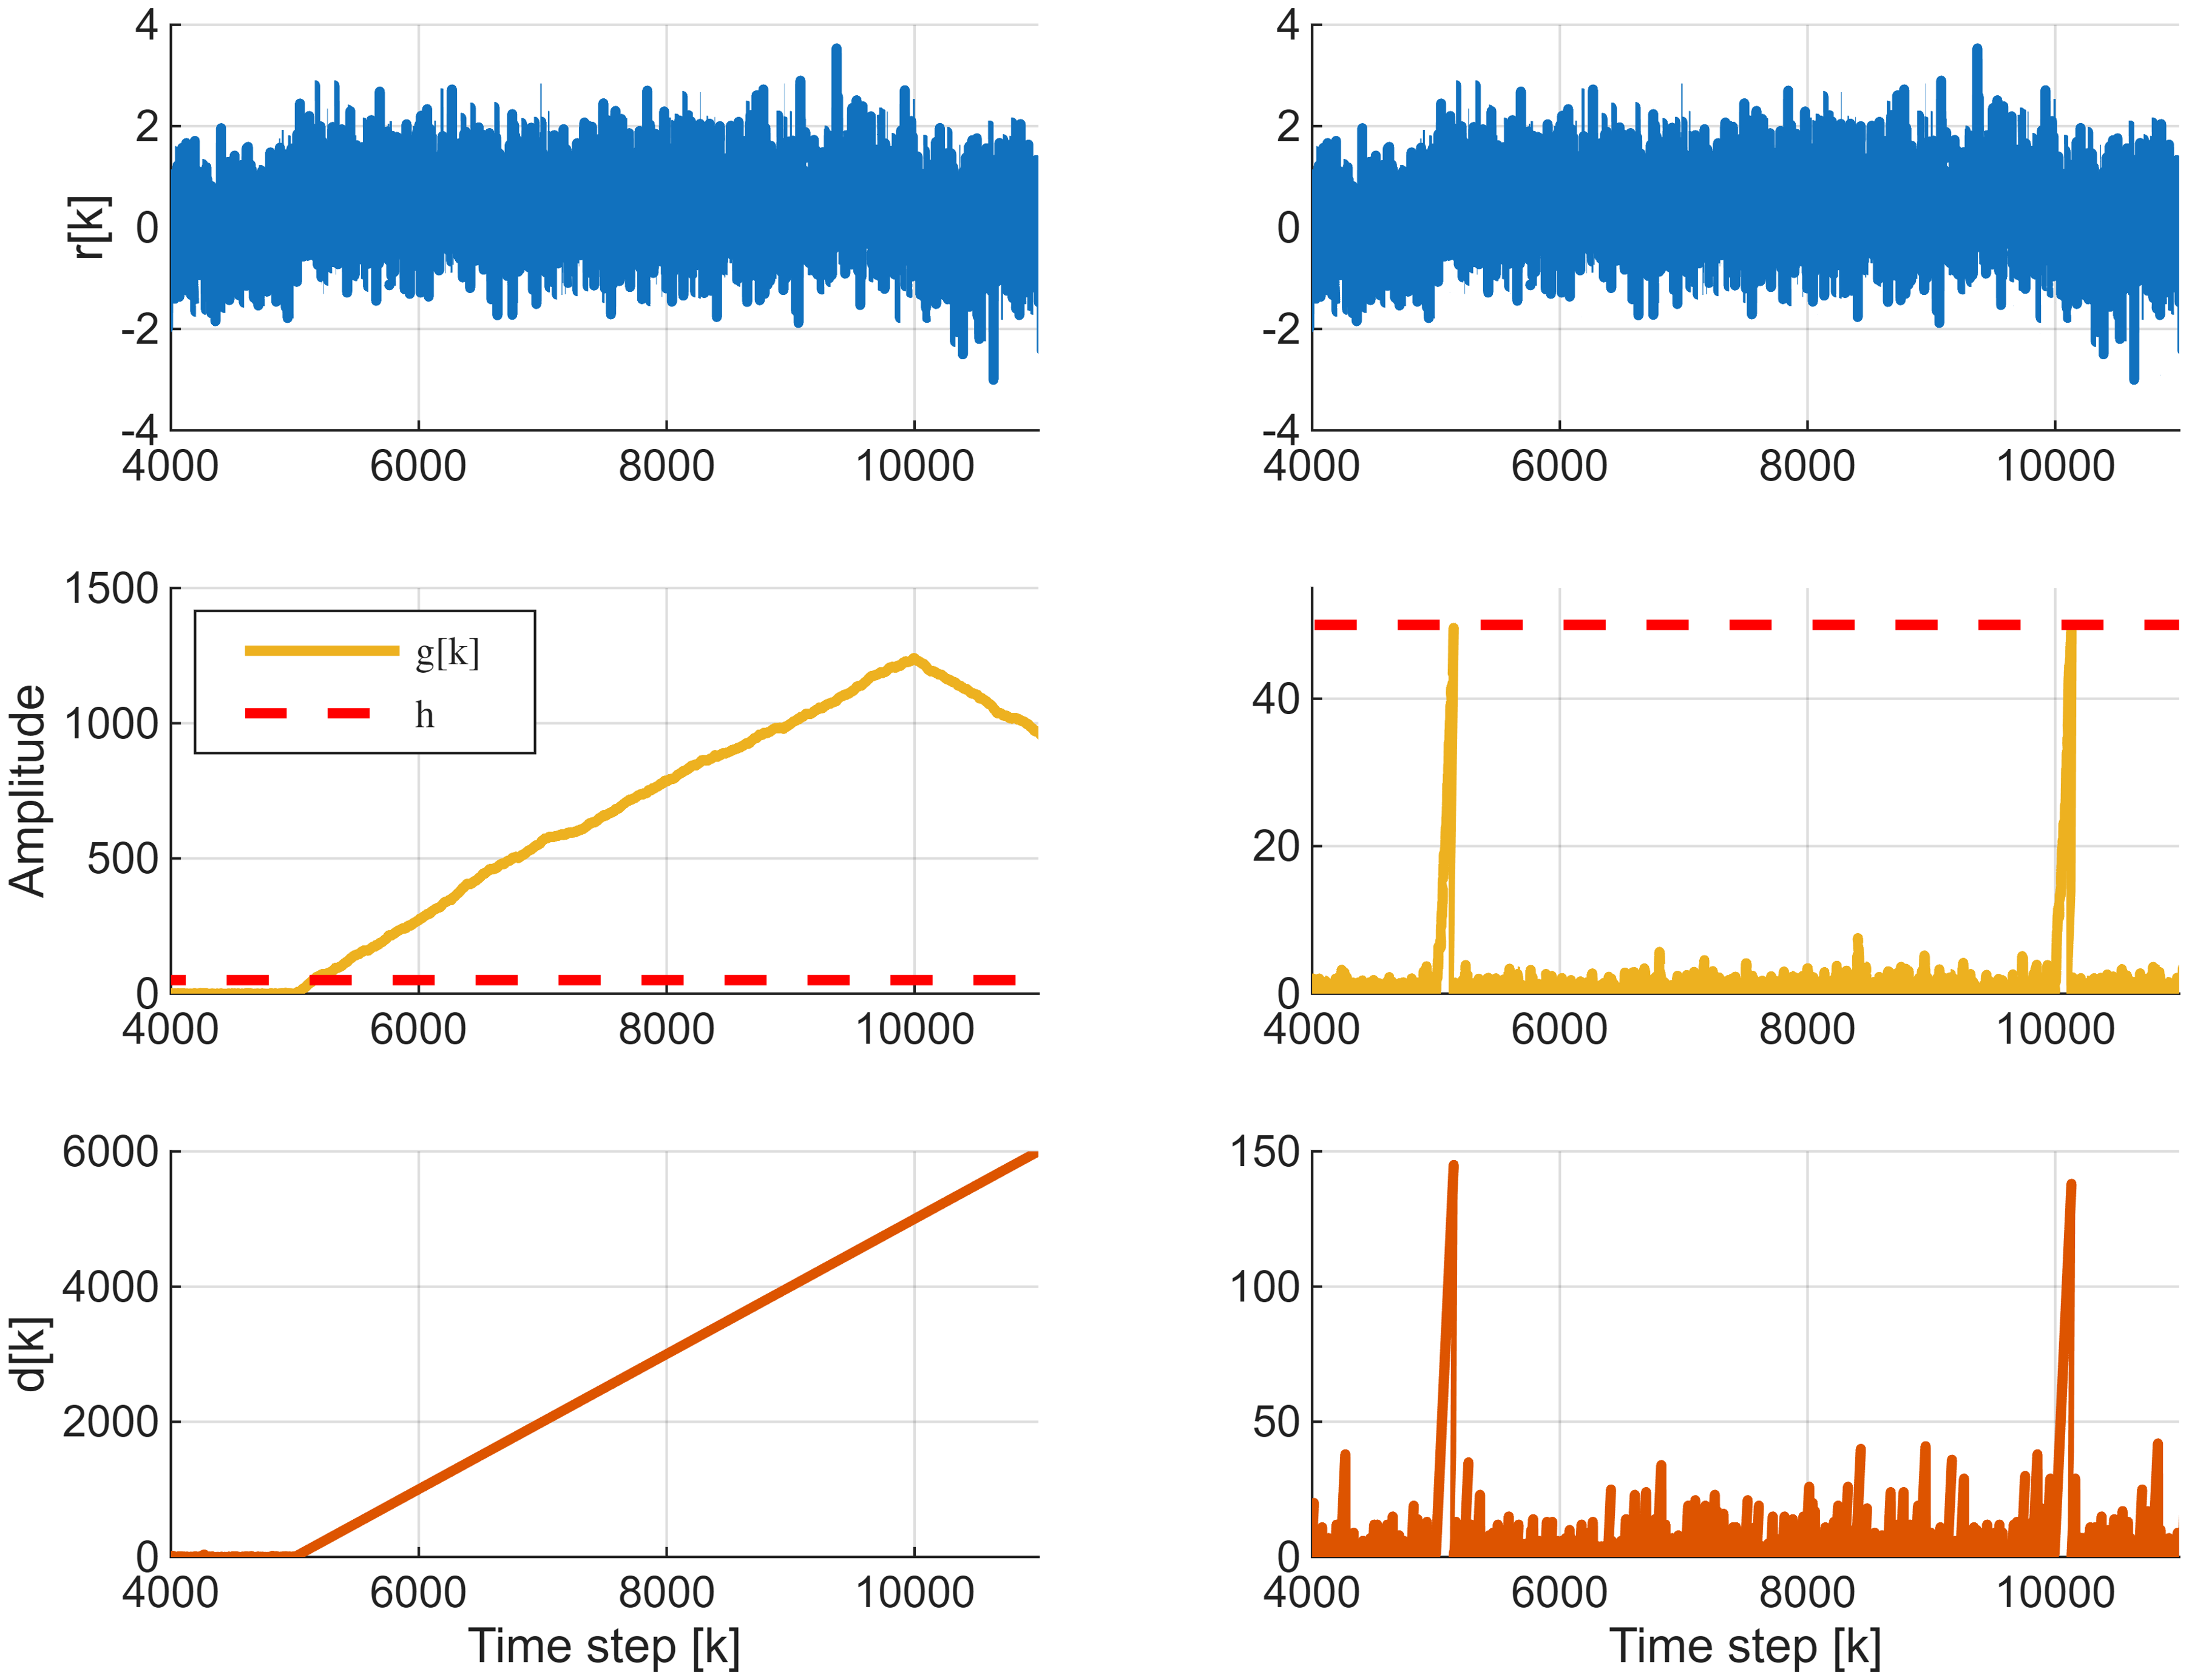
\includegraphics[width=0.48\textwidth]{../Matlab/OnlineChangeDetection/CUSUM.png}
    \caption{CUSUM results for the basic method (left) and the CUSUM with reset (right) for the signal described in Appendix \ref{annex:onlineSystem}}
    \label{fig:CUSUM}
\end{figure}

The left column of Fig.~\ref{fig:CUSUM} shows the fault is indeed detected and the CUSUM algorithm estimates it occurred at sample 4998 instead of 5000. The end of the fault however stays undetected. When there is no fault, $s[k]$ is negative in average as the probability of having no fault is larger than the one of having a fault, meaning $S[k]$ decreases. It is only when it has passed under the threshold $h$ that a new error might be detected again.

The right column of Fig.~\ref{fig:CUSUM} therefore implements a \textit{CUSUM with reset} algorithm, which once a change in the mean is detected change its decision function in order for it to track when the mean goes back to the fault-free value. This is simply done by resetting $g[m]$ to 0 and by replacing $s[k]$ by $-s[k]$, as the minus with the logarithm will invert the probability in (\ref{eq:CUSUM}).

The disappearance of the fault can therefore be detected (at sample 10007 instead of 10000) and the algorithm then resets again to track any new fault.

The computation of $s$ (\ref{eq:CUSUM_s}) however requires the fault amplitude to be known, which is why the GLR on-line criterion is introduced.

\subsection{GLR}

The on-line GLR algorithm choses at each time instant the most likely time of fault occurrence in a window of fixed size $M$. The decision criterion is then computed based on this estimated fault occurrence time $j$, and a fault is detected if it passes above a fixed threshold. The decision criterion $g_{\text{GLR}}$ is expressed as:

\begin{equation}
    g_{\text{GLR}}[k] = \max_{k-M \leq j \leq k} \frac{\left(\sum_{i=j}^{k} (r[i]-m_0)\right)^2}{2\sigma^2 \times \left(k-j+1\right)}
    \label{eq:glrCirtOnline}
\end{equation}

Once a value exceeds the threshold $h$, the maximum likelihood estimate of the amplitude change can be computed using:
\begin{equation}
    \hat{\nu}[k] = \frac{\sum_{i=j}^{k} (r[i]-m_0)}{k-j+1},
\end{equation}
where $j$ is the one that maximized (\ref{eq:glrCirtOnline}). This was tested with different window sizes $M$, and the results are shown on Fig. \ref{fig:GLR_online}.

Compared to the results of the CUSUM algorithm, the detection time is worse as $g[k]$ needs to cross the threshold in order for the GLR to detect the fault. It is however able to detect the amplitude of the fault, making it more robust against unknown faults.

The window size impacts two main parameters: the required threshold and the time to settle after the fault disappears. With the smallest window size, $g[k]$ is relatively close to the threshold even when there is a fault. During the experiments, smaller window sizes $(10, 50)$ had to be removed as they were not able to distinguish faulty and faultless samples. A larger window size allows to chose a larger threshold, but $g[k]$ then takes more time to fall back under the threshold after the fault disappears.

\begin{figure}[htbp]
    \centering
    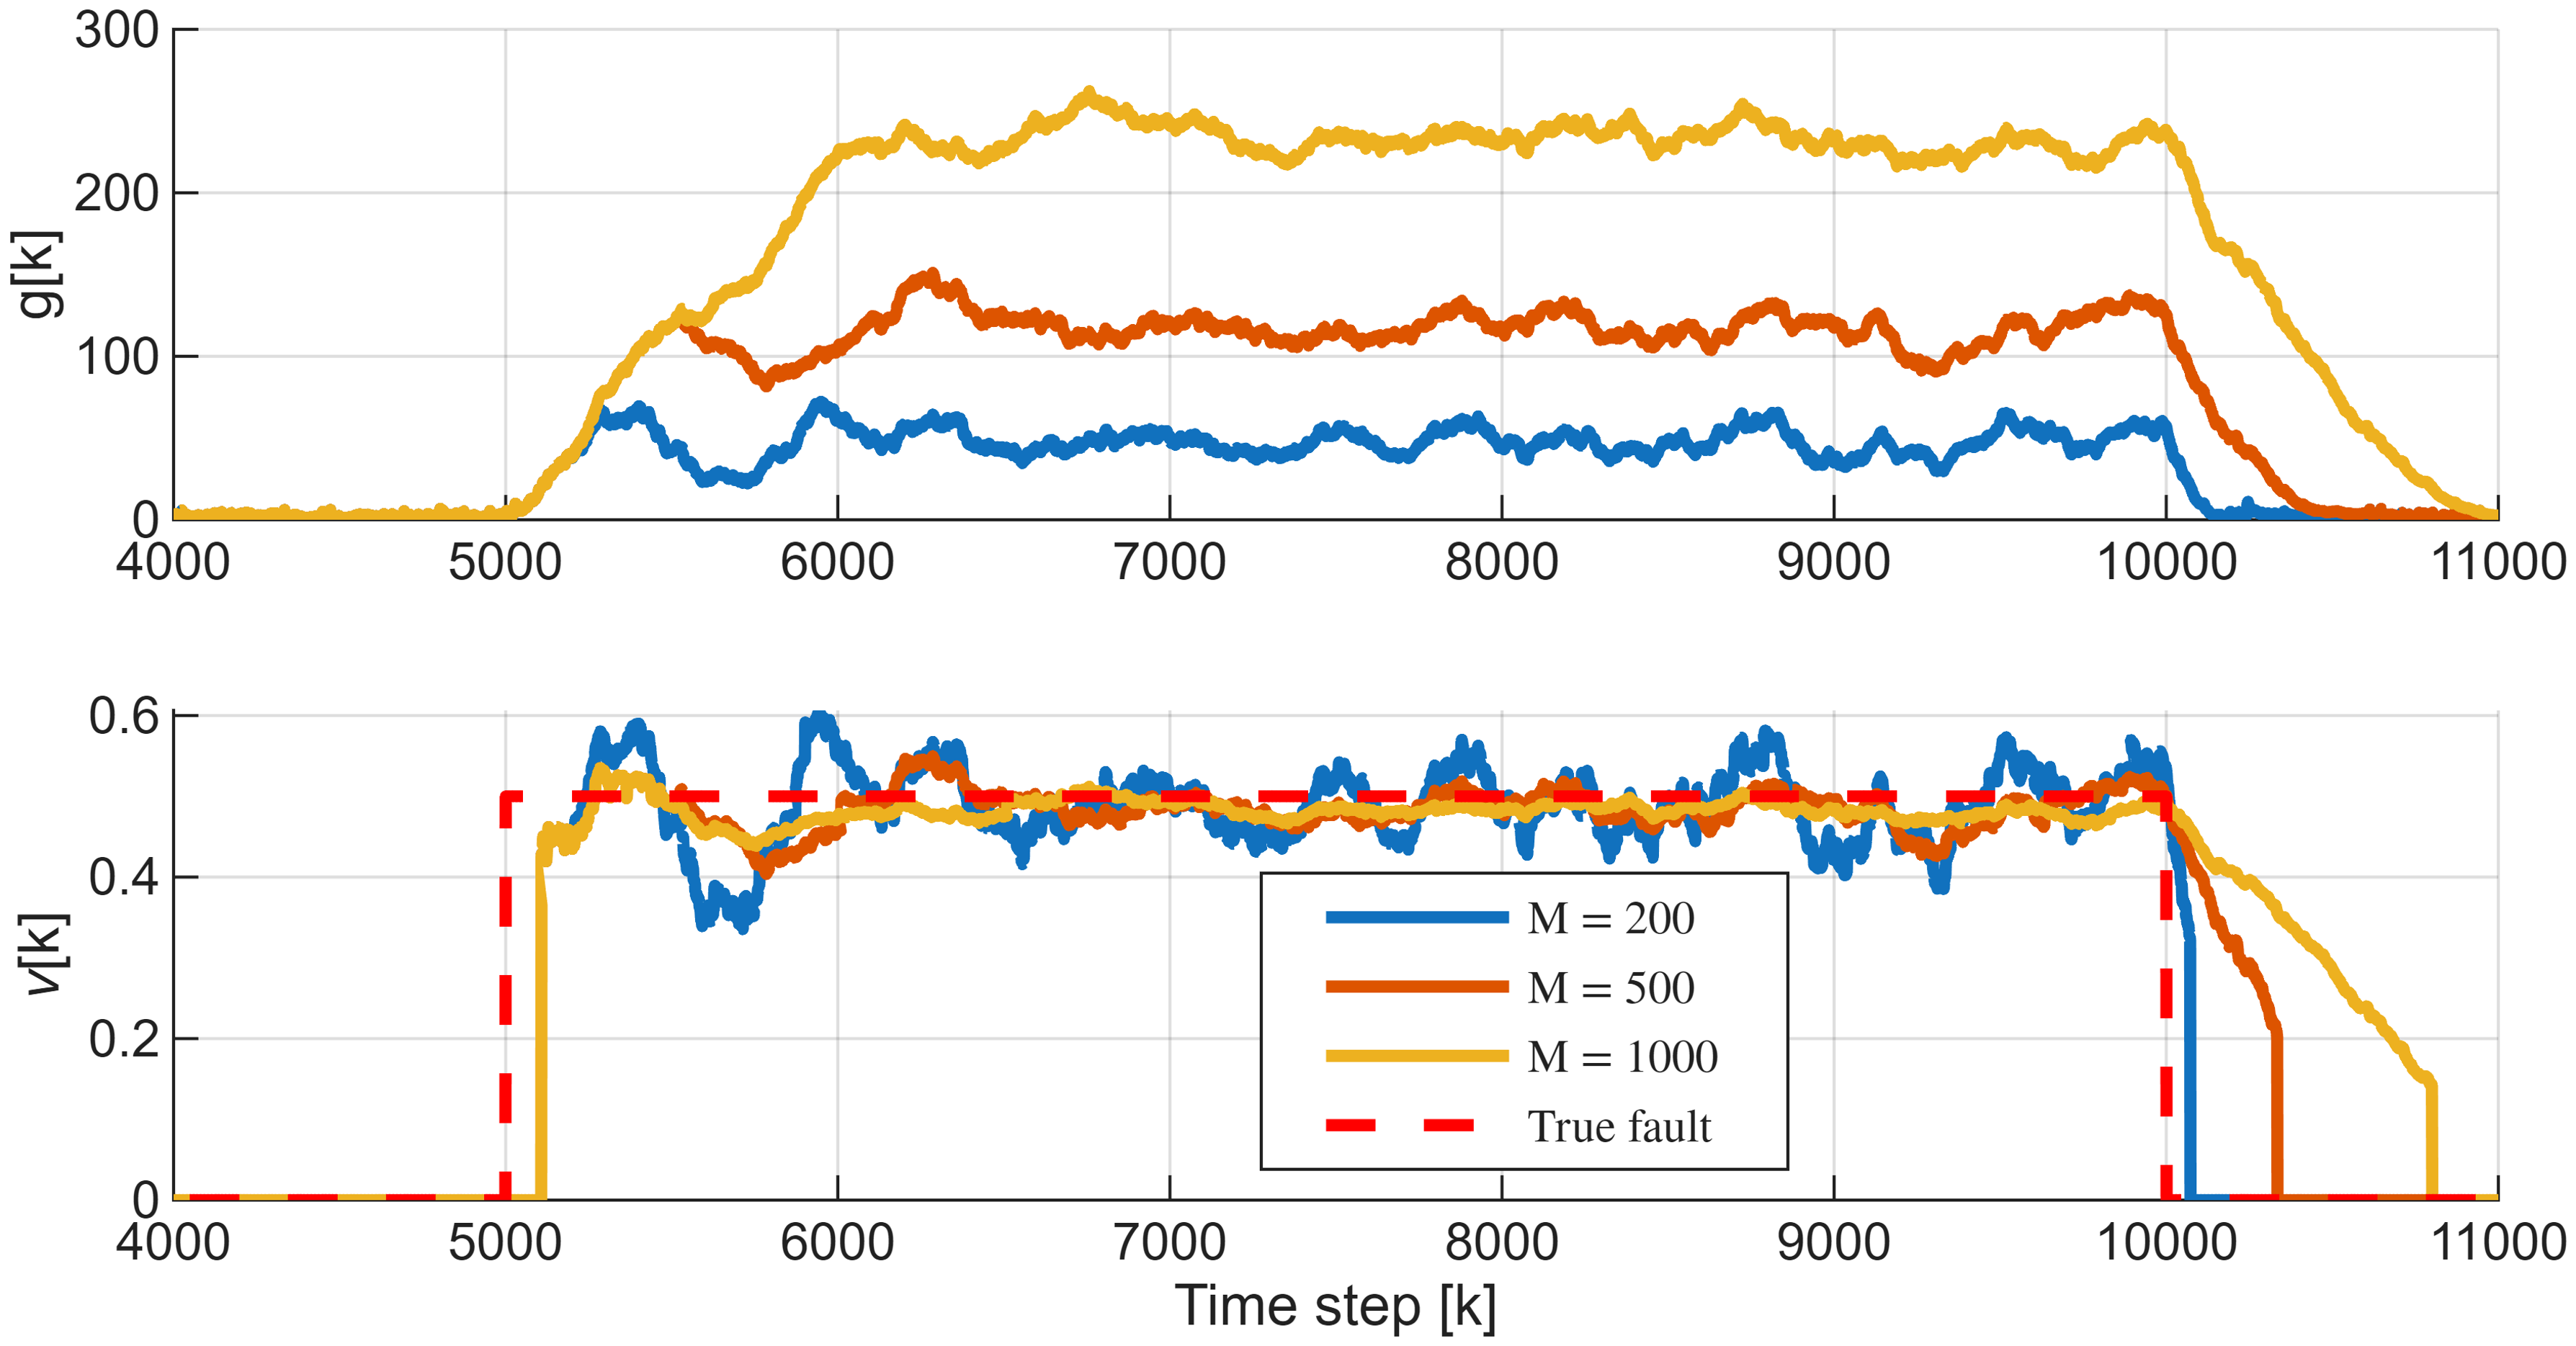
\includegraphics[width=0.48\textwidth]{../Matlab/OnlineChangeDetection/GLR.png}
    \caption{On-line GLR fault detection with different window sizes.}
    \label{fig:GLR_online}
\end{figure}

\appendices
\section{Exact Ship Model}
\label{appendix:exact_model}

The model used in the simulations is, in continuous time,
\begin{equation}
    \dot{x}(t) = A_c x(t) + B_c u(t) + E_{d,c} d(t) + E_{f,c} f(t),
\end{equation}
\begin{equation}
    y(t) = C_c x(t) + D_c u(t) + G_{d,c} d(t) + G_{f,c} f(t),
\end{equation}
with
\begin{equation}
    A_c = \begin{bmatrix}
        b\eta_1 & 0 \\
        1 & 0
    \end{bmatrix},
    \quad
    B_c = \begin{bmatrix}
        b \\
        0
    \end{bmatrix},
    \quad
    E_{d,c} = \begin{bmatrix}
        0 \\
        1
    \end{bmatrix},
\end{equation}
\begin{equation}
    E_{f,c} = \mathbf{0}, \quad \text{and} \quad \begin{cases}
        b = 2.2\\
        \eta_1 = -10
    \end{cases}.
\end{equation}

The output equation matrices are
\begin{equation}
    C_c = \begin{bmatrix}
        1 & 0 \\
        0 & 1
    \end{bmatrix},
    \quad
    D_c = 0,
\end{equation}
\begin{equation}
    G_{d,c} = \begin{bmatrix}
        1 \\
        0
    \end{bmatrix},
    \quad
    G_{f,c} = \begin{bmatrix}
        1 & 0 \\
        0 & 1
    \end{bmatrix}.
\end{equation}

The discrete-time model in (\ref{eq:ss_model}) is finally obtained using a ZOH discretization with sampling time $T_s = 0.2$ seconds.

\section{Three-Phased signal Model}
\label{appendix:three_phased_model}

Fig. \ref{fig:data} shows the signal in a case no fault is applied. Knowing the sampling period $T_s = 1$ms, the frequency of the signal is computed by
\begin{equation}
    \omega_{\text{exc}} = \frac{2 \pi}{50  T_s}
\end{equation}
because there are $50$ measurements per period.

\begin{figure}[htbp]
    \centering
    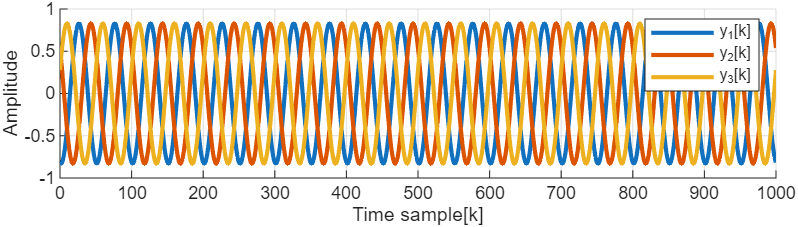
\includegraphics[width=0.48\textwidth]{../Matlab/ObserverMethods/Data.png}
    \caption{Three-phased signal measured by 3 (faultless) sensors.}
    \label{fig:data}
\end{figure}

The continuous-time state space model of this system (which has no input) is given by
\begin{equation}
    \mathbf{\dot{x}} = \begin{bmatrix}
        0 & \omega_{\text{exc}}\\
        -\omega_{\text{exc}} & 0
    \end{bmatrix} \mathbf{x}.
\end{equation}
Because there is an offset between the three phases, the output relationship is expressed as follows, where $\mathbf{f}$ is the fault vector:
\begin{equation}
    \mathbf{y} = \begin{bmatrix}
        \cos(0) & \sin(0)\\
        \cos(\frac{-2 \pi}{3}) & \sin(\frac{-2 \pi}{3}) \\
        \cos(\frac{2 \pi}{3}) & \sin(\frac{2 \pi}{3}) \\
    \end{bmatrix} \mathbf{x} + \mathbf{f}.
\end{equation}

This continuous-time model is then discretized using the ZOH with the known sampling frequency.


\end{document}
